\documentclass[11pt]{article}
\usepackage[utf8]{inputenc}
\usepackage[margin=1in]{geometry}
\usepackage{graphicx}
\usepackage{listings}
\usepackage{xcolor}
\usepackage{booktabs}
\usepackage{array}
\usepackage{tikz}
\usetikzlibrary{shapes.geometric, arrows.meta, positioning, fit}
\usepackage{amsmath}
\usepackage{hyperref}

% Code listing style
\lstdefinestyle{mystyle}{
    backgroundcolor=\color{gray!10},
    commentstyle=\color{green!60!black},
    keywordstyle=\color{blue},
    numberstyle=\tiny\color{gray},
    stringstyle=\color{orange!80!black},
    basicstyle=\ttfamily\footnotesize,
    breakatwhitespace=false,
    breaklines=true,
    captionpos=b,
    keepspaces=true,
    numbers=left,
    numbersep=5pt,
    showspaces=false,
    showstringspaces=false,
    showtabs=false,
    tabsize=2,
    frame=single
}
\lstset{style=mystyle}

\title{Data Structure Overview: \\FALcon-Polygon-SemAIM Pipeline}
\author{}
\date{\today}

\begin{document}

\maketitle

\tableofcontents
\newpage

\section{Introduction}

This document provides a comprehensive overview of the data structure throughout the FALcon-Polygon-SemAIM pipeline. The pipeline processes ImageNet images through three main stages: (1) object detection with FALcon, (2) polygon-based importance score computation, and (3) importance-aware fine-tuning with SemAIM.

\section{Single Image Data Flow}

Figure~\ref{fig:single_image_flow} illustrates how a single image is transformed as it flows through the complete pipeline, showing the specific data structures at each stage.

\begin{figure}[p]
\centering
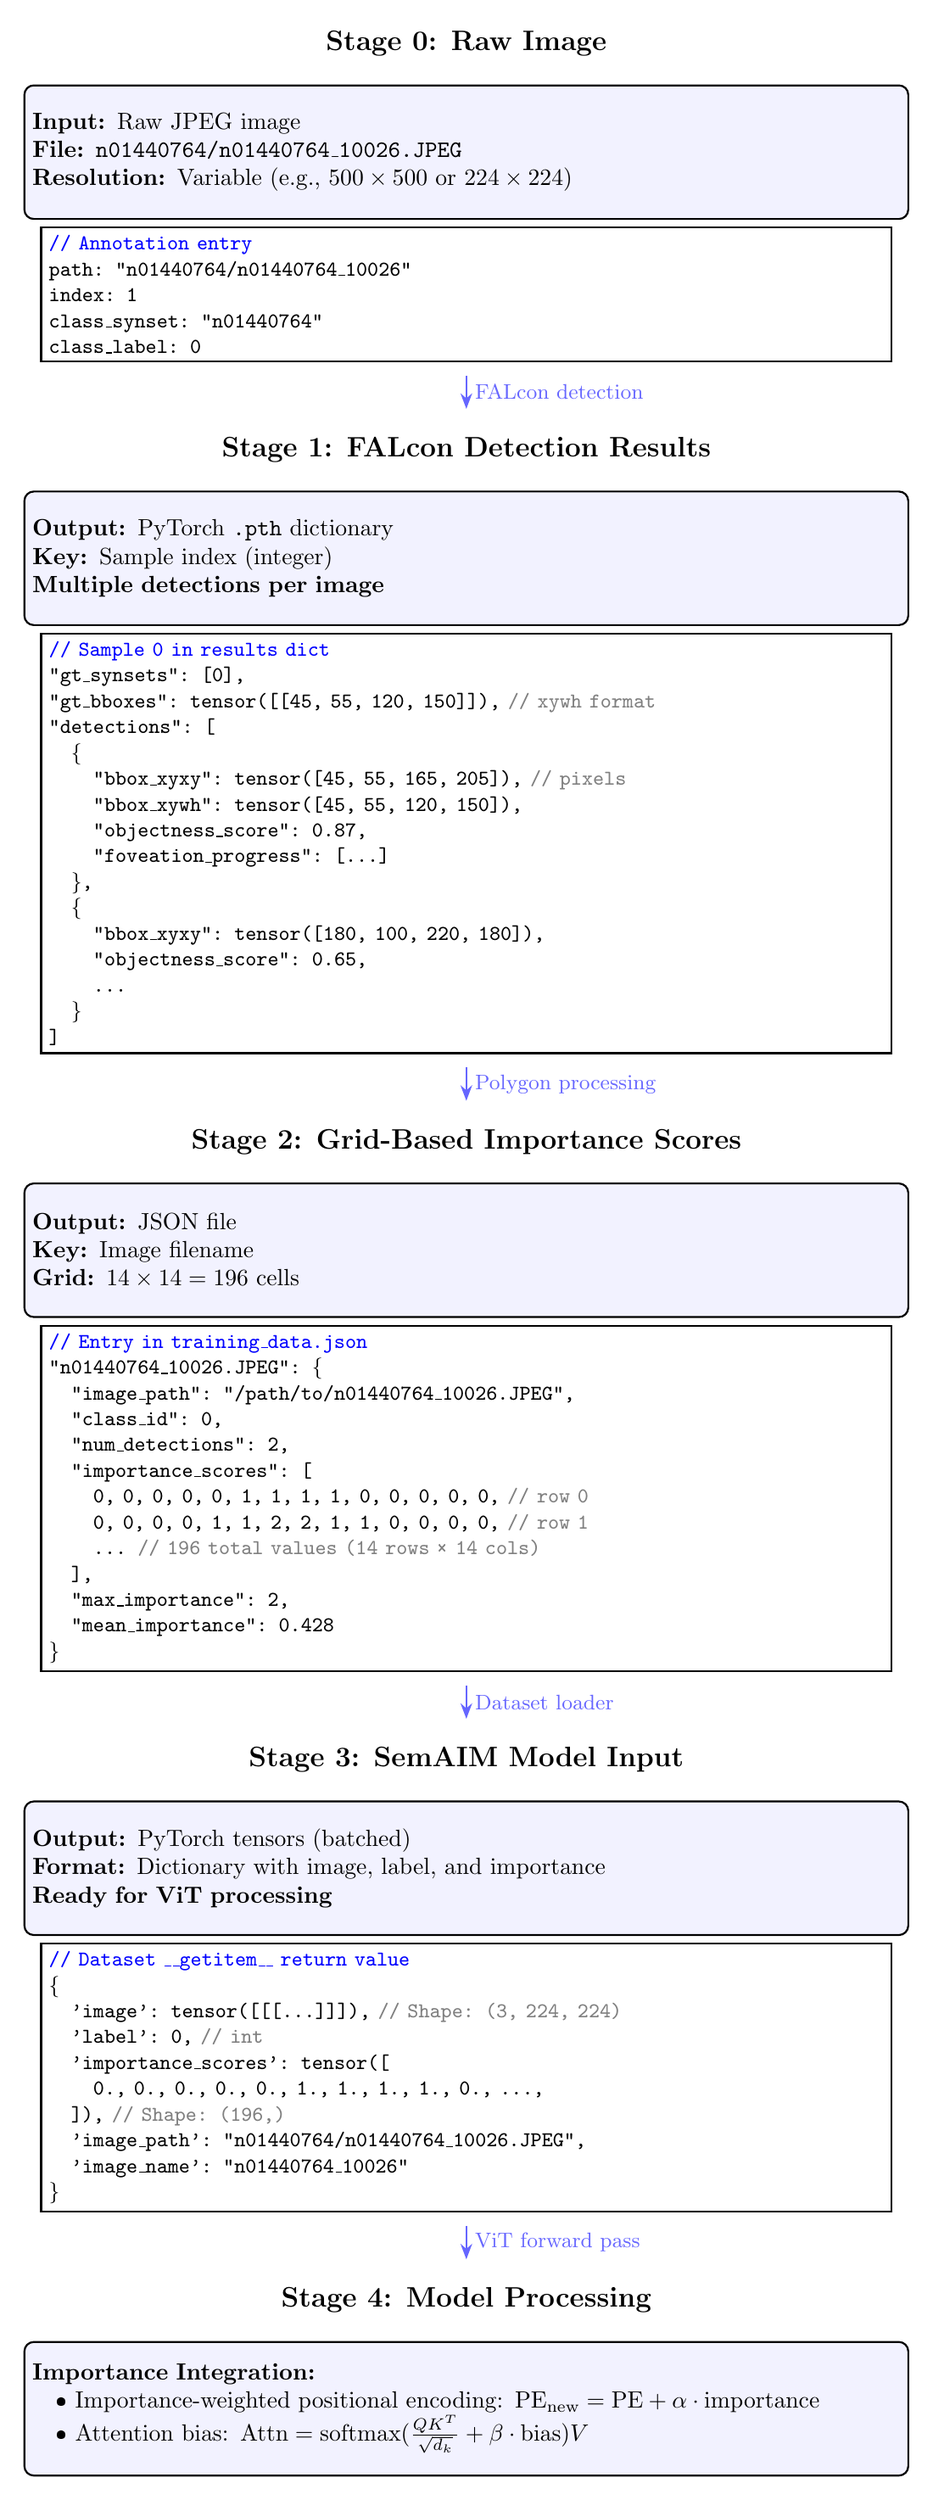
\begin{tikzpicture}[
    node distance=0.3cm,
    stage/.style={rectangle, draw, thick, text width=13cm, align=left, minimum height=2cm, rounded corners, fill=blue!5},
    data/.style={rectangle, draw, thick, text width=12.5cm, align=left, font=\small\ttfamily, fill=white},
    label/.style={font=\bfseries\large},
    arrow/.style={-Stealth, thick, blue!60}
]

% Stage 0: Raw Image
\node[label] (stage0_label) {Stage 0: Raw Image};
\node[stage, below=of stage0_label, anchor=north] (stage0) {
    \textbf{Input:} Raw JPEG image \\
    \textbf{File:} \texttt{n01440764/n01440764\_10026.JPEG} \\
    \textbf{Resolution:} Variable (e.g., $500 \times 500$ or $224 \times 224$)
};
\node[data, below=0.1cm of stage0] (data0) {
    \textcolor{blue}{// Annotation entry} \\
    path: "n01440764/n01440764\_10026" \\
    index: 1 \\
    class\_synset: "n01440764" \\
    class\_label: 0
};

% Arrow
\draw[arrow] ([yshift=-0.2cm]data0.south) -- ++(0,-0.5) node[midway, right, font=\small, text width=3cm] {FALcon detection};

% Stage 1: FALcon Output
\node[label, below=1.0cm of data0] (stage1_label) {Stage 1: FALcon Detection Results};
\node[stage, below=of stage1_label, anchor=north] (stage1) {
    \textbf{Output:} PyTorch \texttt{.pth} dictionary \\
    \textbf{Key:} Sample index (integer) \\
    \textbf{Multiple detections per image}
};
\node[data, below=0.1cm of stage1] (data1) {
    \textcolor{blue}{// Sample 0 in results dict} \\
    "gt\_synsets": [0], \\
    "gt\_bboxes": tensor([[45, 55, 120, 150]]), \textcolor{gray}{// xywh format} \\
    "detections": [ \\
    \quad \{ \\
    \quad\quad "bbox\_xyxy": tensor([45, 55, 165, 205]), \textcolor{gray}{// pixels} \\
    \quad\quad "bbox\_xywh": tensor([45, 55, 120, 150]), \\
    \quad\quad "objectness\_score": 0.87, \\
    \quad\quad "foveation\_progress": [...] \\
    \quad \}, \\
    \quad \{ \\
    \quad\quad "bbox\_xyxy": tensor([180, 100, 220, 180]), \\
    \quad\quad "objectness\_score": 0.65, \\
    \quad\quad ... \\
    \quad \} \\
    ]
};

% Arrow
\draw[arrow] ([yshift=-0.2cm]data1.south) -- ++(0,-0.5) node[midway, right, font=\small, text width=3cm] {Polygon processing};

% Stage 2: Polygon Processing
\node[label, below=1.0cm of data1] (stage2_label) {Stage 2: Grid-Based Importance Scores};
\node[stage, below=of stage2_label, anchor=north] (stage2) {
    \textbf{Output:} JSON file \\
    \textbf{Key:} Image filename \\
    \textbf{Grid:} $14 \times 14 = 196$ cells
};
\node[data, below=0.1cm of stage2] (data2) {
    \textcolor{blue}{// Entry in training\_data.json} \\
    "n01440764\_10026.JPEG": \{ \\
    \quad "image\_path": "/path/to/n01440764\_10026.JPEG", \\
    \quad "class\_id": 0, \\
    \quad "num\_detections": 2, \\
    \quad "importance\_scores": [ \\
    \quad\quad 0, 0, 0, 0, 0, 1, 1, 1, 1, 0, 0, 0, 0, 0, \textcolor{gray}{// row 0} \\
    \quad\quad 0, 0, 0, 0, 1, 1, 2, 2, 1, 1, 0, 0, 0, 0, \textcolor{gray}{// row 1} \\
    \quad\quad ... \textcolor{gray}{// 196 total values (14 rows × 14 cols)} \\
    \quad ], \\
    \quad "max\_importance": 2, \\
    \quad "mean\_importance": 0.428 \\
    \}
};

% Arrow
\draw[arrow] ([yshift=-0.2cm]data2.south) -- ++(0,-0.5) node[midway, right, font=\small, text width=3cm] {Dataset loader};

% Stage 3: SemAIM Input
\node[label, below=1.0cm of data2] (stage3_label) {Stage 3: SemAIM Model Input};
\node[stage, below=of stage3_label, anchor=north] (stage3) {
    \textbf{Output:} PyTorch tensors (batched) \\
    \textbf{Format:} Dictionary with image, label, and importance \\
    \textbf{Ready for ViT processing}
};
\node[data, below=0.1cm of stage3] (data3) {
    \textcolor{blue}{// Dataset \_\_getitem\_\_ return value} \\
    \{ \\
    \quad 'image': tensor([[[...]]]),  \textcolor{gray}{// Shape: (3, 224, 224)} \\
    \quad 'label': 0, \textcolor{gray}{// int} \\
    \quad 'importance\_scores': tensor([ \\
    \quad\quad 0., 0., 0., 0., 0., 1., 1., 1., 1., 0., ..., \\
    \quad ]),  \textcolor{gray}{// Shape: (196,)} \\
    \quad 'image\_path': "n01440764/n01440764\_10026.JPEG", \\
    \quad 'image\_name': "n01440764\_10026" \\
    \}
};

% Arrow
\draw[arrow] ([yshift=-0.2cm]data3.south) -- ++(0,-0.5) node[midway, right, font=\small, text width=3cm] {ViT forward pass};

% Stage 4: Model Processing
\node[label, below=1.0cm of data3] (stage4_label) {Stage 4: Model Processing};
\node[stage, below=of stage4_label, anchor=north] (stage4) {
    \textbf{Importance Integration:} \\
    \quad • Importance-weighted positional encoding: $\text{PE}_{\text{new}} = \text{PE} + \alpha \cdot \text{importance}$ \\
    \quad • Attention bias: $\text{Attn} = \text{softmax}(\frac{QK^T}{\sqrt{d_k}} + \beta \cdot \text{bias})V$
};

\end{tikzpicture}
\caption{Single image data transformation through the complete pipeline. Each stage shows the exact data structure for image \texttt{n01440764\_10026.JPEG} as it progresses from raw input to model-ready tensors.}
\label{fig:single_image_flow}
\end{figure}

\clearpage

\section{Pipeline Overview}

\subsection{Global Architecture}

The complete pipeline consists of four main stages:

\begin{enumerate}
    \item \textbf{Raw ImageNet Data}: Original images with class labels
    \item \textbf{FALcon Detection}: VGG-based object localization with foveation
    \item \textbf{Polygon Processing}: Conversion to grid-based importance scores
    \item \textbf{SemAIM Training}: Importance-aware Vision Transformer fine-tuning
\end{enumerate}

\subsection{Data Flow Diagram}

\begin{figure}[h]
\centering
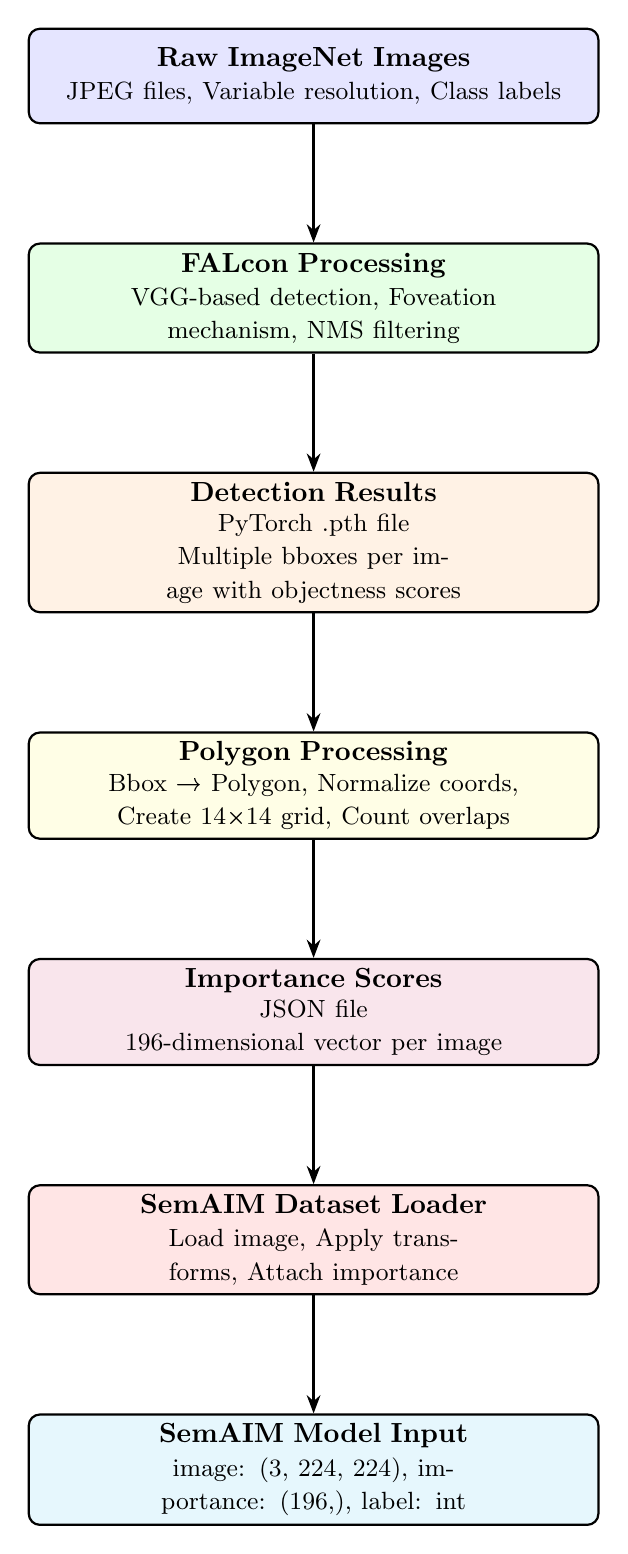
\begin{tikzpicture}[
    node distance=1.5cm,
    box/.style={rectangle, draw, thick, text width=7cm, align=center, minimum height=1.2cm, rounded corners},
    arrow/.style={-Stealth, thick}
]

% Nodes
\node[box, fill=blue!10] (raw) {
    \textbf{Raw ImageNet Images} \\
    \small JPEG files, Variable resolution, Class labels
};

\node[box, fill=green!10, below=of raw] (falcon) {
    \textbf{FALcon Processing} \\
    \small VGG-based detection, Foveation mechanism, NMS filtering
};

\node[box, fill=orange!10, below=of falcon] (detections) {
    \textbf{Detection Results} \\
    \small PyTorch .pth file \\
    \small Multiple bboxes per image with objectness scores
};

\node[box, fill=yellow!10, below=of detections] (polygon) {
    \textbf{Polygon Processing} \\
    \small Bbox → Polygon, Normalize coords, \\
    \small Create 14×14 grid, Count overlaps
};

\node[box, fill=purple!10, below=of polygon] (importance) {
    \textbf{Importance Scores} \\
    \small JSON file \\
    \small 196-dimensional vector per image
};

\node[box, fill=red!10, below=of importance] (loader) {
    \textbf{SemAIM Dataset Loader} \\
    \small Load image, Apply transforms, Attach importance
};

\node[box, fill=cyan!10, below=of loader] (model) {
    \textbf{SemAIM Model Input} \\
    \small image: (3, 224, 224), importance: (196,), label: int
};

% Arrows
\draw[arrow] (raw) -- (falcon);
\draw[arrow] (falcon) -- (detections);
\draw[arrow] (detections) -- (polygon);
\draw[arrow] (polygon) -- (importance);
\draw[arrow] (importance) -- (loader);
\draw[arrow] (loader) -- (model);

\end{tikzpicture}
\caption{Data flow through the complete pipeline}
\label{fig:dataflow}
\end{figure}

\newpage

\section{Stage 1: Initial Data (Raw ImageNet)}

\subsection{Location}
\begin{verbatim}
/home/20204130/imagenet-subset/ILSVRC/Data/CLS-LOC/train/
\end{verbatim}

\subsection{Directory Structure}

\begin{lstlisting}[language=bash, caption=ImageNet directory structure]
train/
├── n01440764/
│   ├── n01440764_10026.JPEG
│   ├── n01440764_10027.JPEG
│   └── ...
├── n01443537/
│   ├── n01443537_*.JPEG
│   └── ...
└── ...
\end{lstlisting}

\subsection{Annotation Format}

Annotation file: \texttt{train\_cls.txt}

\begin{lstlisting}[language=bash, caption=Annotation file format]
n01440764/n01440764_10026 1
n01440764/n01440764_10027 2
n01440764/n01440764_10029 3
...
\end{lstlisting}

\noindent Format: \texttt{<class\_id>/<image\_name> <index>}

\subsection{Data Fields}

\begin{table}[h]
\centering
\begin{tabular}{>{\raggedright}p{3cm}p{10cm}}
\toprule
\textbf{Field} & \textbf{Description} \\
\midrule
Images & Standard JPEG images with variable resolutions \\
Class labels & Synset IDs (e.g., 'n01440764') \\
Index mapping & Line number in annotation file → image path \\
\bottomrule
\end{tabular}
\caption{Raw ImageNet data fields}
\end{table}

\newpage

\section{Stage 2: FALcon Output (Object Detection Results)}

\subsection{Location}
\begin{verbatim}
Falcon/FALcon-main/results/imagenet/.../
imagenet_localization_only_from1to6500.pth
\end{verbatim}

\subsection{File Format}

PyTorch \texttt{.pth} file containing a nested dictionary structure.

\subsection{Data Structure}

\begin{lstlisting}[language=Python, caption=FALcon output structure]
{
    sample_idx: {
        "gt_synsets": [target_class],          # List[int]
        "gt_bboxes": torch.Tensor,             # Shape: (N, 4) - xywh
        "detections": [                         # List of dicts
            {
                "bbox_xywh": torch.Tensor,      # Shape: (4,)
                "bbox_xyxy": torch.Tensor,      # Shape: (4,)
                "objectness_score": float,      # Range: [0.0, 1.0]
                "foveation_progress": [...]     # List[Tensor]
            },
            # ... more detections
        ]
    },
    # ... more samples
}
\end{lstlisting}

\subsection{Bounding Box Formats}

\begin{table}[h]
\centering
\begin{tabular}{>{\raggedright}p{3cm}>{\raggedright}p{10cm}}
\toprule
\textbf{Format} & \textbf{Description} \\
\midrule
\texttt{bbox\_xywh} & $[x, y, \text{width}, \text{height}]$ where $(x,y)$ is top-left corner \\
\texttt{bbox\_xyxy} & $[x_1, y_1, x_2, y_2]$ where $(x_1,y_1)$ is top-left and $(x_2,y_2)$ is bottom-right \\
\bottomrule
\end{tabular}
\caption{Bounding box coordinate formats}
\end{table}

\subsection{Key Characteristics}

\begin{itemize}
    \item \textbf{Multiple detections}: Each image can have 0 to $N$ bounding boxes
    \item \textbf{Pixel coordinates}: Full resolution coordinates (e.g., 224×224 or 500×500)
    \item \textbf{Objectness scores}: Confidence values from FALcon's attention mechanism, range $[0, 1]$
    \item \textbf{Foveation trajectory}: Sequence of bounding boxes showing iterative refinement
\end{itemize}

\subsection{Example Data}

\begin{lstlisting}[language=Python, caption=Example FALcon output for one image]
Sample 42: {
    "gt_synsets": [1],
    "gt_bboxes": tensor([[50, 60, 120, 150]]),  # xywh format
    "detections": [
        {
            "bbox_xyxy": tensor([45, 55, 165, 205]),
            "bbox_xywh": tensor([45, 55, 120, 150]),
            "objectness_score": 0.87,
            "foveation_progress": [...]
        },
        {
            "bbox_xyxy": tensor([180, 100, 220, 180]),
            "bbox_xywh": tensor([180, 100, 40, 80]),
            "objectness_score": 0.65,
            "foveation_progress": [...]
        }
    ]
}
\end{lstlisting}

\newpage

\section{Stage 3: Polygon Processing (Importance Score Generation)}

\subsection{Location}
\begin{verbatim}
Falcon/Polygon/results_vis/training_data_output/training_data.json
\end{verbatim}

\subsection{File Format}

JSON file with per-image importance scores.

\subsection{Data Structure}

\begin{lstlisting}[language=Python, caption=Polygon processing output structure]
{
  "n01440764_10026.JPEG": {
    "image_path": "/path/to/image.JPEG",
    "class_id": 1,
    "num_detections": 2,
    "importance_scores": [0, 0, 1, 2, 2, 1, 0, ...],  // 196 values
    "max_importance": 2,
    "mean_importance": 0.428
  },
  ...
}
\end{lstlisting}

\subsection{Transformation Process}

The polygon processing stage converts bounding boxes into grid-based importance scores through the following steps:

\begin{enumerate}
    \item \textbf{Bounding boxes → Normalized polygons}: Convert pixel coordinates to normalized $[0, 1]$ space
    \begin{equation}
        x_{\text{norm}} = \frac{x_{\text{pixel}}}{\text{image\_width}}, \quad
        y_{\text{norm}} = \frac{y_{\text{pixel}}}{\text{image\_height}}
    \end{equation}

    \item \textbf{Polygon union}: Merge multiple detections using \texttt{shapely.ops.unary\_union}

    \item \textbf{Grid overlay}: Create a $14 \times 14$ grid (196 patches for $224 \times 224$ images)

    \item \textbf{Intersection counting}: For each grid cell, count overlapping detections
    \begin{equation}
        \text{importance}(i) = \sum_{j=1}^{N_{\text{det}}} \mathbb{1}[\text{cell}_i \cap \text{detection}_j \neq \emptyset]
    \end{equation}
\end{enumerate}

\subsection{Grid Structure}

\begin{table}[h]
\centering
\begin{tabular}{ll}
\toprule
\textbf{Parameter} & \textbf{Value} \\
\midrule
Grid size & $14 \times 14 = 196$ tokens \\
Patch size & $16 \times 16$ pixels (for $224 \times 224$ images) \\
Coordinate system & Normalized $[0, 1]$ range \\
Token indexing & $\text{token\_idx} = \text{row} \times 14 + \text{col}$ \\
\bottomrule
\end{tabular}
\caption{Grid structure parameters}
\end{table}

\subsection{Importance Score Semantics}

\begin{table}[h]
\centering
\begin{tabular}{>{\centering}p{2cm}p{10cm}}
\toprule
\textbf{Score} & \textbf{Interpretation} \\
\midrule
0 & No detection overlap (background region) \\
1 & One detection overlaps this cell (normal importance) \\
$\geq 2$ & Multiple detections overlap (high importance region) \\
\bottomrule
\end{tabular}
\caption{Importance score interpretation}
\end{table}

\subsection{Grid Visualization}

\begin{figure}[h]
\centering
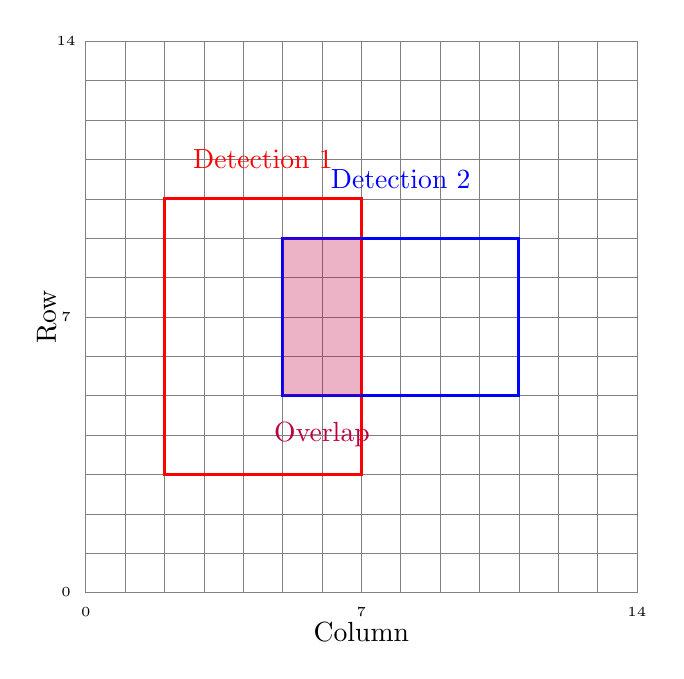
\begin{tikzpicture}[scale=0.5]
    % Draw grid
    \draw[step=1cm,gray,very thin] (0,0) grid (14,14);

    % Draw bounding box 1 (red)
    \draw[red, very thick] (2,3) rectangle (7,10);
    \node[red] at (4.5, 11) {Detection 1};

    % Draw bounding box 2 (blue)
    \draw[blue, very thick] (5,5) rectangle (11,9);
    \node[blue] at (8, 10.5) {Detection 2};

    % Highlight overlap region
    \fill[purple, opacity=0.3] (5,5) rectangle (7,9);
    \node[purple] at (6, 4) {Overlap};

    % Add labels
    \node at (7, -1) {Column};
    \node[rotate=90] at (-1, 7) {Row};

    % Add coordinate labels
    \foreach \x in {0,7,14}
        \node at (\x, -0.5) {\tiny \x};
    \foreach \y in {0,7,14}
        \node at (-0.5, \y) {\tiny \y};
\end{tikzpicture}
\caption{Example of two detections on a $14 \times 14$ grid. Red and blue regions have importance score 1, purple overlap region has importance score 2.}
\end{figure}

\subsection{Complete Data File}

In addition to the minimal training data, a complete data file is also generated containing:

\begin{itemize}
    \item Unified polygon (GeoJSON format)
    \item Individual detection polygons with metadata
    \item Ground truth bounding boxes in pixel coordinates
    \item Per-detection objectness scores
\end{itemize}

\newpage

\section{Stage 4: SemAIM Input (Fine-tuning Dataset)}

\subsection{Location}
\begin{verbatim}
SemAIM/SemAIM-master/datasets/dataset_finetune_importance.py
\end{verbatim}

\subsection{Dataset Loader}

The \texttt{ImageNetWithImportanceFinetune} class loads images with their precomputed importance scores.

\subsection{Output Format}

\begin{lstlisting}[language=Python, caption=SemAIM dataset loader output]
{
    'image': torch.Tensor,           # Shape: (3, 224, 224)
    'label': int,                    # Class label (0-4 for 5 classes)
    'importance_scores': torch.Tensor,  # Shape: (196,)
    'image_path': str,              # e.g., "n01440764/n01440764_10026.JPEG"
    'image_name': str               # e.g., "n01440764_10026"
}
\end{lstlisting}

\subsection{Preprocessing Pipeline}

\subsubsection{Image Transformations (Training)}

\begin{enumerate}
    \item Random resized crop
    \item Random horizontal flip
    \item Color jitter
    \item AutoAugment (\texttt{rand-m9-mstd0.5-inc1})
    \item ToTensor: Convert PIL Image to tensor, scale to $[0, 1]$
    \item Normalize using ImageNet statistics:
    \begin{align}
        \mu &= [0.485, 0.456, 0.406] \\
        \sigma &= [0.229, 0.224, 0.225]
    \end{align}
\end{enumerate}

\subsubsection{Image Transformations (Validation)}

\begin{enumerate}
    \item Resize to 256
    \item Center crop to 224
    \item ToTensor
    \item Normalize (same as training)
\end{enumerate}

\subsection{Importance Score Integration}

The importance scores are integrated into the Vision Transformer through two mechanisms:

\subsubsection{Importance-Weighted Positional Encoding}

\begin{equation}
\text{PE}_{\text{new}}(i) = \text{PE}_{\text{original}}(i) + \alpha \cdot \text{importance}(i)
\end{equation}

where $\alpha$ is a scaling hyperparameter (default: 1.0).

\subsubsection{Attention Bias}

An additional bias term is added to the self-attention mechanism:

\begin{equation}
\text{Attention}(Q, K, V) = \text{softmax}\left(\frac{QK^T}{\sqrt{d_k}} + \beta \cdot \text{importance\_bias}\right)V
\end{equation}

where $\beta$ is a scaling hyperparameter (default: 0.1).

\subsection{Fallback Strategy}

If an image does not have precomputed importance scores:

\begin{equation}
\text{importance\_scores} = \mathbf{1}_{196} = [1, 1, \ldots, 1]
\end{equation}

This ensures uniform attention across all patches (standard ViT behavior).

\newpage

\section{Data Transformation Summary}

\subsection{Coordinate System Transformations}

\begin{table}[h]
\centering
\begin{tabular}{>{\raggedright}p{4cm}>{\raggedright\arraybackslash}p{9cm}}
\toprule
\textbf{Stage} & \textbf{Coordinate System} \\
\midrule
Raw bounding boxes (FALcon) & Pixel coordinates at full resolution \\
& Example: $[45, 55, 165, 205]$ for $224 \times 224$ image \\[0.5em]
Normalized polygons (Polygon) & Normalized $[0, 1]$ range \\
& Example: $[0.2, 0.245, 0.736, 0.915]$ \\[0.5em]
Grid indices (SemAIM) & Flat index $\{0, 1, \ldots, 195\}$ for $14 \times 14$ grid \\
\bottomrule
\end{tabular}
\caption{Coordinate system transformations across pipeline stages}
\end{table}

\subsection{Data Type Transformations}

\begin{table}[h]
\centering
\begin{tabular}{>{\raggedright}p{3cm}>{\raggedright}p{5cm}>{\raggedright\arraybackslash}p{5cm}}
\toprule
\textbf{Stage} & \textbf{Format} & \textbf{Key Type} \\
\midrule
FALcon output & PyTorch \texttt{.pth} & \texttt{torch.Tensor} \\
Polygon processing & JSON & Python \texttt{list}, \texttt{dict} \\
SemAIM loader & PyTorch Dataset & \texttt{torch.Tensor} \\
\bottomrule
\end{tabular}
\caption{Data format transformations}
\end{table}

\subsection{Dimensionality Transformations}

\begin{figure}[h]
\centering
\begin{tikzpicture}[node distance=2cm]
    \node[box] (det) {
        \textbf{Detections} \\
        $N$ boxes $\times$ 4 coords \\
        Variable $N$
    };

    \node[box, right=of det] (poly) {
        \textbf{Polygons} \\
        $N$ polygons \\
        Normalized coords
    };

    \node[box, right=of poly] (grid) {
        \textbf{Grid Scores} \\
        $14 \times 14 = 196$ \\
        Integer counts
    };

    \node[box, right=of grid] (model) {
        \textbf{Model Input} \\
        Vector: (196,) \\
        Float tensor
    };

    \draw[arrow] (det) -- (poly);
    \draw[arrow] (poly) -- (grid);
    \draw[arrow] (grid) -- (model);
\end{tikzpicture}
\caption{Dimensionality transformation from variable detections to fixed-size importance vector}
\end{figure}

\newpage

\section{Implementation Details}

\subsection{Key Files}

\begin{table}[h]
\centering
\small
\begin{tabular}{>{\raggedright}p{6cm}>{\raggedright\arraybackslash}p{7cm}}
\toprule
\textbf{File} & \textbf{Purpose} \\
\midrule
\texttt{FALcon\_collect\_samples\_imagenet\_without\_CLS.py} & Generate detections from FALcon model \\[0.3em]
\texttt{json\_processing.py} & Process pseudo-bbox annotations \\[0.3em]
\texttt{final\_polygon\_v2.py} & Convert detections to importance scores \\[0.3em]
\texttt{dataset\_finetune\_importance.py} & PyTorch dataset loader for SemAIM \\[0.3em]
\texttt{main\_finetune\_importance.py} & Training script for importance-aware ViT \\[0.3em]
\bottomrule
\end{tabular}
\caption{Key implementation files}
\end{table}

\subsection{Grid Cell to Token Index Mapping}

For a $14 \times 14$ grid with row-major ordering:

\begin{equation}
\text{token\_idx}(\text{row}, \text{col}) = \text{row} \times 14 + \text{col}
\end{equation}

Inverse mapping:

\begin{align}
\text{row} &= \lfloor \text{token\_idx} / 14 \rfloor \\
\text{col} &= \text{token\_idx} \mod 14
\end{align}

\subsection{Importance Score Statistics}

Typical distribution across a dataset:

\begin{table}[h]
\centering
\begin{tabular}{>{\centering}p{3cm}>{\centering}p{3cm}>{\centering\arraybackslash}p{5cm}}
\toprule
\textbf{Score} & \textbf{Percentage} & \textbf{Interpretation} \\
\midrule
0 & 60-70\% & Background cells \\
1 & 25-35\% & Object cells \\
$\geq 2$ & 5-10\% & Multi-object overlap cells \\
\bottomrule
\end{tabular}
\caption{Typical importance score distribution}
\end{table}

\section{Usage Example}

\subsection{Loading FALcon Results}

\begin{lstlisting}[language=Python, caption=Load FALcon detection results]
import torch

# Load detection results
results = torch.load('imagenet_localization_only_from1to6500.pth')

# Access sample 0
sample = results[0]
print(f"Number of detections: {len(sample['detections'])}")

# Access first detection
det = sample['detections'][0]
print(f"BBox (xyxy): {det['bbox_xyxy']}")
print(f"Objectness: {det['objectness_score']:.3f}")
\end{lstlisting}

\subsection{Loading Importance Scores}

\begin{lstlisting}[language=Python, caption=Load importance scores]
import json

# Load importance data
with open('training_data.json', 'r') as f:
    importance_data = json.load(f)

# Access sample
img_name = "n01440764_10026.JPEG"
scores = importance_data[img_name]['importance_scores']
print(f"Importance scores shape: {len(scores)}")  # 196
print(f"Max importance: {max(scores)}")
\end{lstlisting}

\subsection{Using SemAIM Dataset}

\begin{lstlisting}[language=Python, caption=Use SemAIM dataset loader]
from datasets.dataset_finetune_importance import \
    ImageNetWithImportanceFinetune
from torch.utils.data import DataLoader

# Create dataset
dataset = ImageNetWithImportanceFinetune(
    root='/path/to/images/train',
    ann_file='/path/to/train.txt',
    importance_file='/path/to/training_data.json',
    transform=transform_train
)

# Create dataloader
loader = DataLoader(dataset, batch_size=64, shuffle=True)

# Iterate
for batch in loader:
    images = batch['image']           # (B, 3, 224, 224)
    labels = batch['label']           # (B,)
    importance = batch['importance_scores']  # (B, 196)
    break
\end{lstlisting}

\section{Conclusion}

This pipeline transforms raw ImageNet images into importance-augmented training data for Vision Transformers. The key innovation is the conversion of object detection results into grid-based importance scores that guide the model's attention mechanism, enabling more efficient learning by focusing on relevant image regions.

The three-stage transformation ensures:
\begin{itemize}
    \item \textbf{Spatial awareness}: Detection bounding boxes capture object locations
    \item \textbf{Fixed dimensionality}: Grid-based scores provide consistent 196-dim vectors
    \item \textbf{Semantic richness}: Overlap counts indicate region importance
    \item \textbf{Model compatibility}: Seamless integration with ViT architecture
\end{itemize}

\end{document}
